% ****** Start of file apssamp.tex ******
%
%   This file is part of the APS files in the REVTeX 4.1 distribution.
%   Version 4.1r of REVTeX, August 2010
%
%   Copyright (c) 2009, 2010 The American Physical Society.
%
%   See the REVTeX 4 README file for restrictions and more information.
%
% TeX'ing this file requires that you have AMS-LaTeX 2.0 installed
% as well as the rest of the prerequisites for REVTeX 4.1
%
% See the REVTeX 4 README file
% It also requires running BibTeX. The commands are as follows:
%
%  1)  latex apssamp.tex
%  2)  bibtex apssamp
%  3)  latex apssamp.tex
%  4)  latex apssamp.tex
%
\documentclass[%
 reprint,
%superscriptaddress,
%groupedaddress,
%unsortedaddress,
%runinaddress,
%frontmatterverbose,
%preprint,
%showpacs,preprintnumbers,
%nofootinbib,
%nobibnotes,
%bibnotes,
amsmath,amssymb,
%aps,
pra,
%prb,
%rmp,
%prstab,
%prstper,
%floatfix,
]{revtex4-1}

\usepackage{siunitx}
\usepackage{graphicx}% Include figure files
\usepackage{dcolumn}% Align table columns on decimal point
\usepackage{bm}% bold math
%\usepackage{hyperref}% add hypertext capabilities
%\usepackage[mathlines]{lineno}% Enable numbering of text and display math
%\linenumbers\relax % Commence numbering lines

%\usepackage[showframe,%Uncomment any one of the following lines to test
%%scale=0.7, marginratio={1:1, 2:3}, ignoreall,% default settings
%%text={7in,10in},centering,
%%margin=1.5in,
%%total={6.5in,8.75in}, top=1.2in, left=0.9in, includefoot,
%%height=10in,a5paper,hmargin={3cm,0.8in},
%]{geometry}

\begin{document}

\preprint{APS/123-QED}

\title{Fabrication and characterization of a Pseudo-MOSFET}% Force line breaks with \\

\author{Moritz Berger}
 \altaffiliation[]{RWTH Aachen University, Germany}%Lines break automatically or can be forced with \\
 \email{moritz.berger@rwth-aachen.de}
 \author{Gerald Kolter}
 \altaffiliation[]{RWTH Aachen University, Germany}%Lines break automatically or can be forced with \\
 \email{gerald.kolter@rwth-aachen.de}

\date{\today}% It is always \today, today,
             %  but any date may be explicitly specified

\begin{abstract}
bla
\end{abstract}

\maketitle

\section{Introduction}
In the following the fabrication of a Pseudo-MOSFET ("metallic-oxide-semiconductor-field-effect-transistor") will be described. The next step is a more detailed description of optical lithographie and reactive ion etching. Afterwards an analysis and a discussion of the characterization of the fabricated Pseudo-MOSFET will be given.

\section{Fabrication}

\begin{table}
\centering
\begin{tabular}{|c|c|}
\hline 
Fabrication technology & "UNIBOND" \\ 
\hline 
top Si thickness & \SI{85}{nm} \\ 
\hline 
buried oxide thickness & \SI{145}{nm} \\ 
\hline 
doping type & p-type (Boron) \\ 
\hline 
doping concentration & $1 \times 10^{15}$ \si{\per\cubic\centi\meter} \\ 
\hline 
crystal orientation & (100) \\ 
\hline 
\end{tabular} 
\caption{Specification of the SOI wafer.}
\label{tab:Spec_SOI}
\end{table}

The basis for the MOSFET are SOI (Semiconductor On Insulator) samples, the specifications are listed in table \ref{tab:Spec_SOI}. Si is used as semiconductor and SiO$_2$ as insulator. In a first step an mask for the following etching was defined lithographically. The mesa structuring is done by reactive ion etching with a gas mixture of SF$_6$/O$_2$. For removing the resist an oxygen plasma is used. At next the samples are RCA-cleaned ending with a dip in hydroflourid acid to get a bare silicon surface. The aluminum is deposited in a vacuum. The aluminum layer is structured with optical lithographie and an aluminum etching as which phosphoric acid, nitric acid, acetic acid and water in a volume ratio of 16:1:1:2 is used. 

\section{Theory}
\subsection{Optical Lithographie}

\subsection{Reactive Ion Etching}
\section{Measurement}
\section{Data Analysis}
\section{Results and Discussion}
In the following chapter the characteristic values of the MOSFETs are extracted out of the measurement data. The methods that are used to do this are shown with the help of the data set of device A5 of the lower right quadrant (4-A5). This device has a tunnel length of \SI{200}{\mu m} with an inner radius of \SI{25}{\mu m} and an outer radius of \SI{225}{\mu m}.
\subsection{output characteristics}
\subsection{effective carrier charge density}
For the extraction of the effective carrier charge density $\mu_{eff}$ the $\dfrac{I_d}{\sqrt{g_m}}$-method is used.\\
\\
In a first step the measured drain-current $I_d$ is plotted against the gate-voltage $V_g$ for three different drain-voltages $V_d$ = \SI{0.03}{V}, \SI{0.05}{V} and \SI{0.07}{V} , as seen in figure \ref{fig:linreg1}. Then the point with the highest slope is determined numerically and a linear regression is fitted at a \SI{1}{\volt} area around this point. The resulting straights are also shown in figure \ref{fig:linreg1}.\\
\\
\begin{figure}
\centering
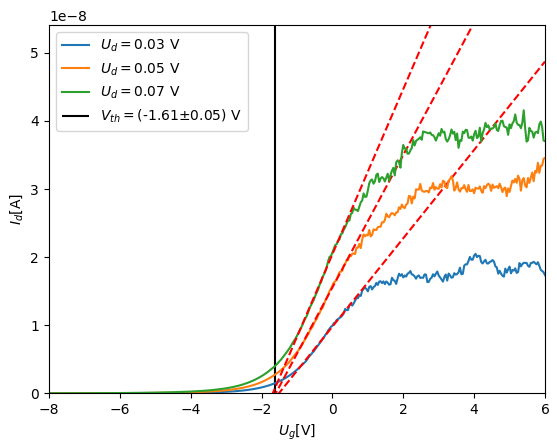
\includegraphics[scale=0.6]{Bilder/linreg.png}
\caption{drain-current $I_d$ plotted against the gate-voltage $V_g$ for different drain Voltages.}
\label{fig:linreg1}
\end{figure}

The threshold-voltage $V_{th}$, as well as its error, can directly be extracted from this fit. This is done for all three curves and a final value for $V_{th}$ for this device is calculated by taking the weighted average of all three values.\\
\\
The slope of this fit is also used to determine $\mu_{eff}$ with the help of the following equation:
\begin{equation}
\sqrt{\mu_{eff} f C_{ox} V_d} \cdot (V_g-V_{th}) = \dfrac{I_d}{\sqrt{g}}
\end{equation}

where $f = 2\pi / ln(R_2/R_1)$ is a structural factor, $C_{ox} = \epsilon_0 \epsilon_{ox} / d_{ox}$ is the capacity of the oxide-layer and g is the slope. $\epsilon_{ox} = 3.9$ is used.\\
In order to get $\mu_{eff}$ out of this $I_d/\sqrt{g}$ is plotted against $V_g$, as seen in figure \ref{fig:linreg2}. A second linear regression is then fitted to this data. From the slope $a$ of this fit one can get $\mu_{eff}$ through:
\begin{equation}
\mu_{eff} = \dfrac{a^2}{f C V_d}
\end{equation}

This is also done for all three drain-voltages. A final value for $\mu_{eff}$ is again calculated by taking the weighted average.

\begin{table}
\centering
\begin{tabular}{|c|c|c|c|}
\hline
$U_d$ & $V_{th}[\si{V}]$ & $g[\si{nA/V}]$ & $mu_{eff}[\si{cm^2/Vs}]$\\
\hline
0.03 & $-1.51\pm 0.02$ & $6.48\pm 0.07$ & $0.59\pm 0.01$\\
\hline
0.05 & $-1.6\pm 0.02$ & $9.72\pm 0.09$ & $0.53\pm 0.0$\\
\hline
0.07 & $-1.69\pm 0.02$ & $12.12\pm 0.1$ & $0.47\pm 0.0$\\
\hline
average & $-1.61\pm 0.05$ & $8.64\pm 1.6$ &$0.51\pm 0.03$\\
\hline
\end{tabular}
\label{tab: exaple_data}
\end{table}



\begin{figure}
\centering
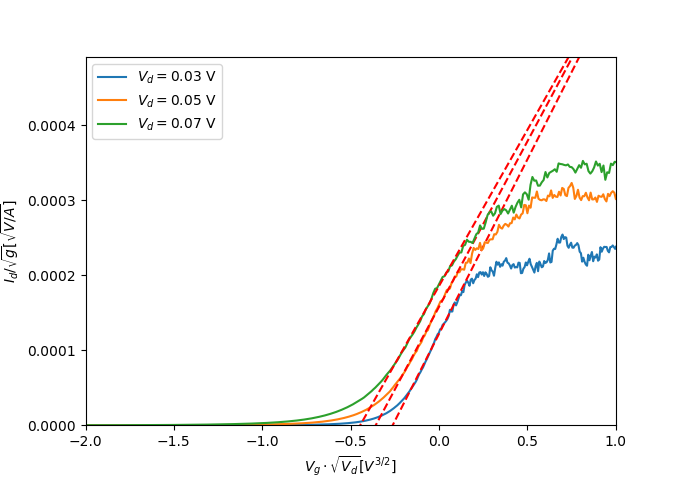
\includegraphics[scale=0.6]{Bilder/mu.png}
\caption{$I_d/\sqrt{g}$ plotted against $V_g \cdot \sqrt{V_d}$ for different drain Voltages.}
\label{fig:linreg2}
\end{figure}


\begin{table}
\centering
\begin{tabular}{|c|c|c|c|c|c|}
\hline 
Position & length & $R_1$ & $R_2$ & $V_{th}$ [\si{\volt}]  & $\mu_{eff}$  [\si{cm^2/Vs}] \\ 
\hline 
3d1 & 50 & 50 & 100 & $-1.28\pm 0.01$ & $5.09\pm 0.07$\\
\hline 
4a1 & 50 & 25 & 75 & $-2.63\pm 0.14$ & $0.21\pm 0.03$\\
\hline 
3e1 & 50 & 150 & 200 & $-0.61\pm 0.01$ & $4.27\pm 0.01$\\
\hline 
\hline 
1b2 & 75 & 50 & 125 & $-0.54\pm 0.02$ & $7.62\pm 0.22$\\
\hline 
1d2 & 75 & 100 & 175 & $-4.29\pm 0.35$ & $0.07\pm 0.01$\\
\hline 
4e2 & 75 & 150 & 225 & $1.31\pm 0.17$ & $0.57\pm 0.04$\\
\hline 
\hline 
4c3 & 150 & 75 & 225 & $-1.51\pm 0.01$ & $0.94\pm 0.02$\\
\hline 
4e3 & 100 & 150 & 250 & $-3.41\pm 2.08$ & $0.04\pm 0.01$\\
\hline 
4b3 & 100 & 50 & 150 & $-4.03\pm 0.05$ & $0.08\pm 0.01$\\
\hline 
\hline 
4c4 & 150 & 75 & 225 & $0.25\pm 0.01$ & $3.0\pm 0.08$\\
\hline 
4e4 & 150 & 150 & 300 & $-5.34\pm 1.73$ & $0.04\pm 0.01$\\
\hline 
4b4 & 150 & 50 & 200 & $-4.9\pm 0.24$ & $0.04\pm 0.01$\\
\hline
4d4 & 150 & 100 & 250 & $-4.08\pm 0.08$ & $0.13\pm 0.01$\\
\hline 
\hline 
4a5 & 200 & 25 & 225 & $-1.61\pm 0.05$ & $2.77\pm 0.17$\\
\hline 
4b5 & 200 & 50 & 250 & $-2.34\pm 0.02$ & $0.85\pm 0.03$\\
\hline 
4c5 & 200 & 75 & 275 & $-3.19\pm 0.22$ & $0.09\pm 0.02$\\
\hline
4d5 & 200 & 100 & 300 & $-1.21\pm 0.02$ & $2.65\pm 0.03$\\
\hline 
4e5 & 200 & 150 & 350 & $-1.56\pm 0.06$ & $1.79\pm 0.1$\\
\hline 

\end{tabular} 
\caption{Results of transfer characterization.}
\label{tab:transfer_results}
\end{table}
\section{Conclusion}

\bibliography{MOSFET}% Produces the bibliography via BibTeX.

\end{document}

\begin{thebibliography}{x}
   \bibitem[Esselborn-Krumbiegel, H., 2008]{bmbf} Von der Idee zum Text. Eine Anleitung zum wissenschaftlichen Schreiben. Paderborn: Verlag Ferdinand Sch�ningh GmbH \& Co. KG.

   \bibitem[Franck, N., 2004]{bmbf} Handbuch Wissenschafliches Arbeiten. Frankfurt am Main: Fischer Taschenbuch Verlag.
Karmasin, M., \& Ribing, R. (2011). Die Gestaltung wissenschaftlicher Arbeiten. Wien: Facultas Verlags- und Buchhandels AG.

   \bibitem[Lengauer, H., \& Wimmer, A., 2006]{bmbf} http://www.uni-klu.ac.at. Abgerufen am 30. 9. 2013 von Definition Plagiat: http://www.uni-klu.ac.at/main/inhalt/3054.htm

   \bibitem[Prei�ner, A., 2012]{bmbf} Wissenschaftliches Arbeiten: Internet nutzen, Text erstellen, �berblick behalten. M�nchen: Oldenbourg.

\end{thebibliography}
